\section{Lecture 4: Statics of Suspension Bridge}
\begin{itemize}
    \item The top-down view of a suspension bridge is seen below:
    \begin{center}
        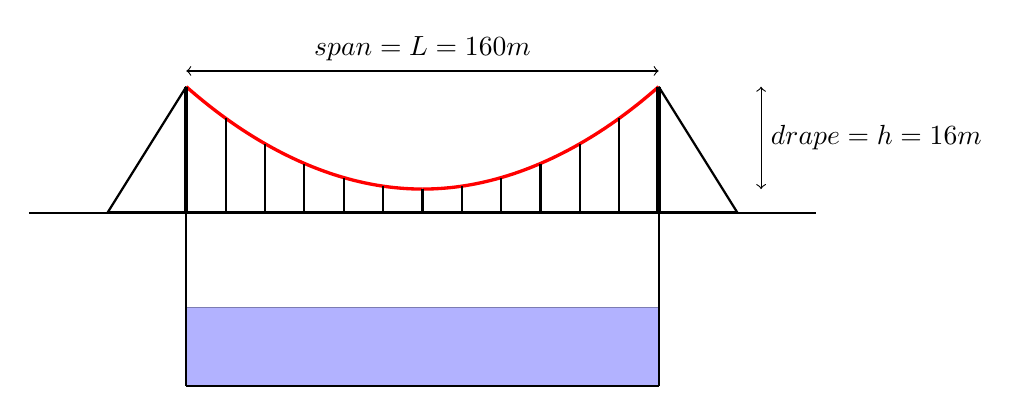
\begin{tikzpicture}
            \draw [fill=blue,opacity=0.3] (-3,1) rectangle (3,0);
            \draw [thick] (-5,2.2)-- (-3,2.2);
            \draw [thick] (-3,2.2)-- (-3,0);
            \draw [thick] (-3,0)-- (3,0);
            \draw [thick] (3,0)-- (3,2.2);
            \draw [thick] (3,2.2)-- (5,2.2);
            
            \draw [color=red,very thick] (0,2.5) parabola (3,3.8);
            \draw [color=red,very thick] (0,2.5) parabola (-3,3.8);
            \draw [very thick] (-4,2.2)-- (4,2.2);

            \foreach \x in {-2.5,-2,...,2.5}
            \draw [thick] (\x ,2.2)-- (\x ,0.144*\x*\x+2.5);

            \draw [ultra thick] (-3 ,2.2)-- (-3,3.8);
            \draw [thick] (-4,2.2) -- (-3,3.8);
            \draw [ultra thick] (3 ,2.2)-- (3,3.8);
            \draw [thick] (4,2.2) -- (3,3.8);
          
            \draw [<->] (-3,4) -- (3,4) node[midway,above] {$\text{span}=L=160\text{ m}$};
            \draw [<->] (4.3,2.5) -- (4.3,3.8) node[midway,right] {$\text{drape}=h=16\text{ m}$};
        \end{tikzpicture}
    \end{center}
    \begin{center}
        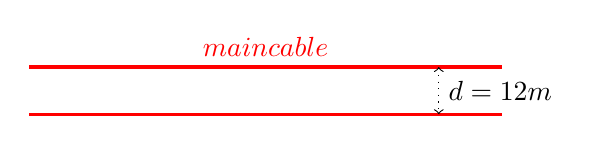
\begin{tikzpicture}
        \draw[color=red,very thick] (-3,0.3) -- (3,0.3) node[midway, above] {$\text{main cable}$};
        \draw[color=red,very thick] (-3,-0.3) -- (3,-0.3);
        \draw[<->,dotted] (2.2,0.3) -- (2.2,-0.3) node[midway,right] {$d=12 \text{ m}$}; 
        \end{tikzpicture}
    \end{center}
    \item We assume that both the live and the dead load is $5 \si{\kilo\newton\per\meter\squared}$ each, which is approximately equivalent to the force exerted by a crowd of people standing close together. We can say that the total weight is $\sigma=10 \si{\kilo\newton\per\meter\squared}$.
    \item We can balance forces on half of the suspension cable:
    \begin{center}
        \begin{tikzpicture}
            
            \draw [color=red,very thick] (0,2.5) parabola (-3,3.8);
            \draw [color=red,dotted] (-3,3.8) -- (-3,2.5) node[midway,right] {$h$};
            \draw [dotted] (-3,3.8) -- (-1.5,3.8) node[midway,above] {$L/4$};

            \draw [thick, ->] (-3,3.8) -- (-4,4.66) node[right] {$F$};
            \draw [dotted, ->] (-4,3.8) -- (-4,4.66) node[midway,left] {$F_y$};
            \draw [dotted, ->] (-3,3.8) -- (-4,3.8) node[midway,below] {$F_y$};

            \draw [thick, ->] (0,2.5) -- (1,2.5) node[above] {$H$};
            \draw [thick, ->] (-1.5,2.82) -- (-1.5,1) node[below] {$V=\sigma\left(\frac{L}{2}d\right)$};
        \end{tikzpicture}
    \end{center}
    And we see that $F_y=V$ and $F_x=H$. We can determine
    \begin{equation}
        V = 9600 \si{\kilo\newton}
        \label{eq:}
    \end{equation}
    These pairs of forces form two couples, so we can determine the magnitude of the forces by summing the moments to zero:
    \begin{equation}
        V\frac{L}{4}=Hh \implies H = \frac{\sigma L^2d}{8h} = 24,000 \si{\kilo\newton}
        \label{eq:}
    \end{equation}
    Therefore, the total force of tension at the top is given by
    \begin{equation}
        F=\sqrt{F_x^2+F_y^2}=12,900 \si{
            \kilo\newton
        }
        \label{eq:}
    \end{equation}
    \item The Golden Gate bridge in San Francisco was an engineering triumph:
    \begin{center}
        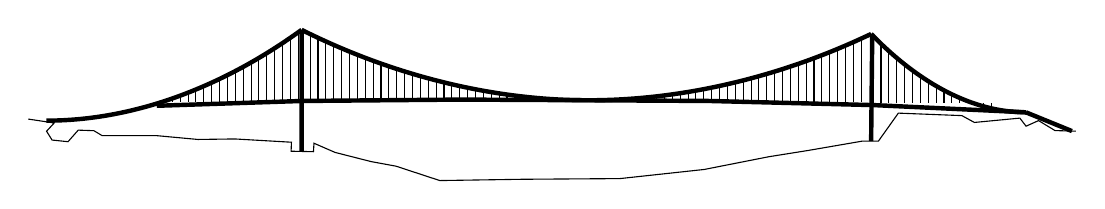
\begin{tikzpicture}[scale=0.5]
            
    \draw [] (-11.26,-3.06)-- (-10.6,-3.159)-- (-10.794,-3.3692)-- (-10.654,-3.5929)-- (-10.249,-3.6348)-- (-9.99,-3.3413)-- (-9.592,-3.355)-- (-9.382,-3.481)-- (-7.998,-3.481)-- (-6.950,-3.578)-- (-6.013,-3.5649)-- (-4.574,-3.648)-- (-4.5828,-3.8767)-- (-4.015,-3.8886)-- (-4.002,-3.6740)-- (-3.4664,-3.907)-- (-2.551,-4.140)-- (-1.9200,-4.256)-- (-0.8059,-4.622)-- (1.3059,-4.589)-- (3.7669,-4.572)-- (5.912,-4.3398)-- (7.549,-4.0169)-- (8.546,-3.858)-- (9.92,-3.6212)-- (10.334,-3.6212)-- (10.841,-2.909)-- (12.455,-2.9723)-- (12.772,-3.146)-- (13.927,-3.0356)-- (14.085,-3.241)-- (14.402,-3.0989)-- (14.82,-3.352)-- (15.352,-3.368);
    \draw [ultra thick] (-7.9959,-2.7228)-- (-4.300,-2.6002)-- (-0.2723,-2.565)-- (2.9676,-2.582)-- (6.032,-2.6002)-- (10.218,-2.7053)-- (14.08,-2.888);
    \draw [ultra thick] (-4.316,-0.7949)-- (-4.317,-3.8823);
    \draw [ultra thick] (10.178,-0.8982)-- (10.150,-3.6212);
    \draw [ultra thick] (15.25,-3.365)-- (14.08,-2.888);
    \draw [ultra thick] (-10.8,-3.1) parabola (-4.316,-0.7949);
    \foreach \x in {-8,-7.8,...,-4.3}
    \draw [] (\x ,-2.62)-- (\x ,0.056*\x*\x+2*10.8*0.056*\x+10.8*10.8*0.056-3.1);
    
    \draw [ultra thick] (2.96768, -2.58274) parabola (-4.316,-0.7949);
    \draw [ultra thick] (2.96768, -2.58274) parabola (10.150,-0.8982);
    \foreach \x in {-4.3,-4.1,...,10}
    \draw [] (\x ,-2.62)-- (\x ,0.033*\x*\x-2*0.033*2.97*\x+0.033*2.97*2.97-2.5827);
    
    
    \draw [ultra thick] (14.08,-2.888) parabola (10.150,-0.8982);
    \foreach \x in {10.2,10.4,...,13.2}
    \draw [] (\x ,-2.65)-- (\x ,0.13*\x*\x+2*-14.08*0.13*\x+14.08*14.08*0.13-2.888);
        \end{tikzpicture}
    \end{center}
    It also revolutionized safety procedures and hugely influenced life in the city. It is sometimes known as the ``Mona Lisa'' of bridges.
    \item The Quebec Bridge, which had a span half of that of the Golden Gate bridge, was not a feat of engineering triumph.
\end{itemize}